\documentclass[1p]{elsarticle_modified}
%\bibliographystyle{elsarticle-num}

%\usepackage[colorlinks]{hyperref}
%\usepackage{abbrmath_seonhwa} %\Abb, \Ascr, \Acal ,\Abf, \Afrak
\usepackage{amsfonts}
\usepackage{amssymb}
\usepackage{amsmath}
\usepackage{amsthm}
\usepackage{scalefnt}
\usepackage{amsbsy}
\usepackage{kotex}
\usepackage{caption}
\usepackage{subfig}
\usepackage{color}
\usepackage{graphicx}
\usepackage{xcolor} %% white, black, red, green, blue, cyan, magenta, yellow
\usepackage{float}
\usepackage{setspace}
\usepackage{hyperref}

\usepackage{tikz}
\usetikzlibrary{arrows}

\usepackage{multirow}
\usepackage{array} % fixed length table
\usepackage{hhline}

%%%%%%%%%%%%%%%%%%%%%
\makeatletter
\renewcommand*\env@matrix[1][\arraystretch]{%
	\edef\arraystretch{#1}%
	\hskip -\arraycolsep
	\let\@ifnextchar\new@ifnextchar
	\array{*\c@MaxMatrixCols c}}
\makeatother %https://tex.stackexchange.com/questions/14071/how-can-i-increase-the-line-spacing-in-a-matrix
%%%%%%%%%%%%%%%

\usepackage[normalem]{ulem}

\newcommand{\msout}[1]{\ifmmode\text{\sout{\ensuremath{#1}}}\else\sout{#1}\fi}
%SOURCE: \msout is \stkout macro in https://tex.stackexchange.com/questions/20609/strikeout-in-math-mode

\newcommand{\cancel}[1]{
	\ifmmode
	{\color{red}\msout{#1}}
	\else
	{\color{red}\sout{#1}}
	\fi
}

\newcommand{\add}[1]{
	{\color{blue}\uwave{#1}}
}

\newcommand{\replace}[2]{
	\ifmmode
	{\color{red}\msout{#1}}{\color{blue}\uwave{#2}}
	\else
	{\color{red}\sout{#1}}{\color{blue}\uwave{#2}}
	\fi
}

\newcommand{\Sol}{\mathcal{S}} %segment
\newcommand{\D}{D} %diagram
\newcommand{\A}{\mathcal{A}} %arc


%%%%%%%%%%%%%%%%%%%%%%%%%%%%%5 test

\def\sl{\operatorname{\textup{SL}}(2,\Cbb)}
\def\psl{\operatorname{\textup{PSL}}(2,\Cbb)}
\def\quan{\mkern 1mu \triangleright \mkern 1mu}

\theoremstyle{definition}
\newtheorem{thm}{Theorem}[section]
\newtheorem{prop}[thm]{Proposition}
\newtheorem{lem}[thm]{Lemma}
\newtheorem{ques}[thm]{Question}
\newtheorem{cor}[thm]{Corollary}
\newtheorem{defn}[thm]{Definition}
\newtheorem{exam}[thm]{Example}
\newtheorem{rmk}[thm]{Remark}
\newtheorem{alg}[thm]{Algorithm}

\newcommand{\I}{\sqrt{-1}}
\begin{document}

%\begin{frontmatter}
%
%\title{Boundary parabolic representations of knots up to 8 crossings}
%
%%% Group authors per affiliation:
%\author{Yunhi Cho} 
%\address{Department of Mathematics, University of Seoul, Seoul, Korea}
%\ead{yhcho@uos.ac.kr}
%
%
%\author{Seonhwa Kim} %\fnref{s_kim}}
%\address{Center for Geometry and Physics, Institute for Basic Science, Pohang, 37673, Korea}
%\ead{ryeona17@ibs.re.kr}
%
%\author{Hyuk Kim}
%\address{Department of Mathematical Sciences, Seoul National University, Seoul 08826, Korea}
%\ead{hyukkim@snu.ac.kr}
%
%\author{Seokbeom Yoon}
%\address{Department of Mathematical Sciences, Seoul National University, Seoul, 08826,  Korea}
%\ead{sbyoon15@snu.ac.kr}
%
%\begin{abstract}
%We find all boundary parabolic representation of knots up to 8 crossings.
%
%\end{abstract}
%\begin{keyword}
%    \MSC[2010] 57M25 
%\end{keyword}
%
%\end{frontmatter}

%\linenumbers
%\tableofcontents
%
\newcommand\colored[1]{\textcolor{white}{\rule[-0.35ex]{0.8em}{1.4ex}}\kern-0.8em\color{red} #1}%
%\newcommand\colored[1]{\textcolor{white}{ #1}\kern-2.17ex	\textcolor{white}{ #1}\kern-1.81ex	\textcolor{white}{ #1}\kern-2.15ex\color{red}#1	}

{\Large $\underline{12a_{0736}~(K12a_{0736})}$}

\setlength{\tabcolsep}{10pt}
\renewcommand{\arraystretch}{1.6}
\vspace{1cm}\begin{tabular}{m{100pt}>{\centering\arraybackslash}m{274pt}}
\multirow{5}{120pt}{
	\centering
	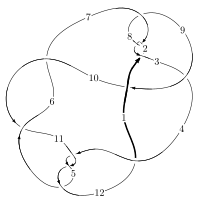
\includegraphics[width=112pt]{../../../GIT/diagram.site/Diagrams/png/1537_12a_0736.png}\\
\ \ \ A knot diagram\footnotemark}&
\allowdisplaybreaks
\textbf{Linearized knot diagam} \\
\cline{2-2}
 &
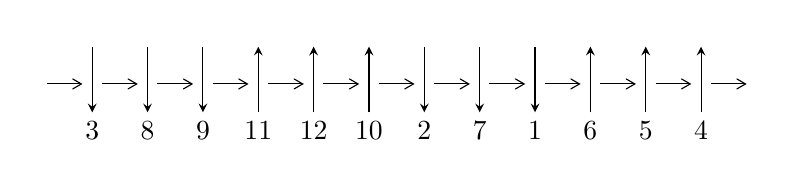
\begin{tikzpicture}[x=20pt, y=17pt]
	% nodes
	\node (C0) at (0, 0) {};
	\node (C1) at (1, 0) {};
	\node (C1U) at (1, +1) {};
	\node (C1D) at (1, -1) {3};

	\node (C2) at (2, 0) {};
	\node (C2U) at (2, +1) {};
	\node (C2D) at (2, -1) {8};

	\node (C3) at (3, 0) {};
	\node (C3U) at (3, +1) {};
	\node (C3D) at (3, -1) {9};

	\node (C4) at (4, 0) {};
	\node (C4U) at (4, +1) {};
	\node (C4D) at (4, -1) {11};

	\node (C5) at (5, 0) {};
	\node (C5U) at (5, +1) {};
	\node (C5D) at (5, -1) {12};

	\node (C6) at (6, 0) {};
	\node (C6U) at (6, +1) {};
	\node (C6D) at (6, -1) {10};

	\node (C7) at (7, 0) {};
	\node (C7U) at (7, +1) {};
	\node (C7D) at (7, -1) {2};

	\node (C8) at (8, 0) {};
	\node (C8U) at (8, +1) {};
	\node (C8D) at (8, -1) {7};

	\node (C9) at (9, 0) {};
	\node (C9U) at (9, +1) {};
	\node (C9D) at (9, -1) {1};

	\node (C10) at (10, 0) {};
	\node (C10U) at (10, +1) {};
	\node (C10D) at (10, -1) {6};

	\node (C11) at (11, 0) {};
	\node (C11U) at (11, +1) {};
	\node (C11D) at (11, -1) {5};

	\node (C12) at (12, 0) {};
	\node (C12U) at (12, +1) {};
	\node (C12D) at (12, -1) {4};
	\node (C13) at (13, 0) {};

	% arrows
	\draw[->,>={angle 60}]
	(C0) edge (C1) (C1) edge (C2) (C2) edge (C3) (C3) edge (C4) (C4) edge (C5) (C5) edge (C6) (C6) edge (C7) (C7) edge (C8) (C8) edge (C9) (C9) edge (C10) (C10) edge (C11) (C11) edge (C12) (C12) edge (C13) ;	\draw[->,>=stealth]
	(C1U) edge (C1D) (C2U) edge (C2D) (C3U) edge (C3D) (C4D) edge (C4U) (C5D) edge (C5U) (C6D) edge (C6U) (C7U) edge (C7D) (C8U) edge (C8D) (C9U) edge (C9D) (C10D) edge (C10U) (C11D) edge (C11U) (C12D) edge (C12U) ;
	\end{tikzpicture} \\
\hhline{~~} \\& 
\textbf{Solving Sequence} \\ \cline{2-2} 
 &
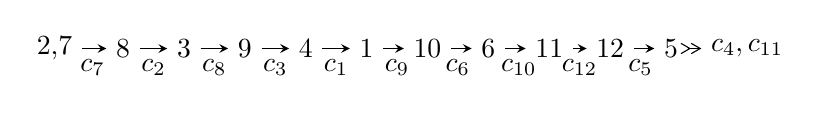
\begin{tikzpicture}[x=22pt, y=7pt]
	% node
	\node (A0) at (-1/8, 0) {2,7};
	\node (A1) at (1, 0) {8};
	\node (A2) at (2, 0) {3};
	\node (A3) at (3, 0) {9};
	\node (A4) at (4, 0) {4};
	\node (A5) at (5, 0) {1};
	\node (A6) at (6, 0) {10};
	\node (A7) at (7, 0) {6};
	\node (A8) at (8, 0) {11};
	\node (A9) at (9, 0) {12};
	\node (A10) at (10, 0) {5};
	\node (C1) at (1/2, -1) {$c_{7}$};
	\node (C2) at (3/2, -1) {$c_{2}$};
	\node (C3) at (5/2, -1) {$c_{8}$};
	\node (C4) at (7/2, -1) {$c_{3}$};
	\node (C5) at (9/2, -1) {$c_{1}$};
	\node (C6) at (11/2, -1) {$c_{9}$};
	\node (C7) at (13/2, -1) {$c_{6}$};
	\node (C8) at (15/2, -1) {$c_{10}$};
	\node (C9) at (17/2, -1) {$c_{12}$};
	\node (C10) at (19/2, -1) {$c_{5}$};
	\node (A11) at (45/4, 0) {$c_{4},c_{11}$};

	% edge
	\draw[->,>=stealth]	
	(A0) edge (A1) (A1) edge (A2) (A2) edge (A3) (A3) edge (A4) (A4) edge (A5) (A5) edge (A6) (A6) edge (A7) (A7) edge (A8) (A8) edge (A9) (A9) edge (A10) ;
	\draw[->>,>={angle 60}]	
	(A10) edge (A11);
\end{tikzpicture} \\ 

\end{tabular} \\

\footnotetext{
The image of knot diagram is generated by the software ``\textbf{Draw programme}" developed by Andrew Bartholomew(\url{http://www.layer8.co.uk/maths/draw/index.htm\#Running-draw}), where we modified some parts for our purpose(\url{https://github.com/CATsTAILs/LinksPainter}).
}\phantom \\ \newline 
\centering \textbf{Ideals for irreducible components\footnotemark of $X_{\text{par}}$} 
 
\begin{align*}
I^u_{1}&=\langle 
u^{69}-11 u^{67}+\cdots+2 u^2+1\rangle \\
I^u_{2}&=\langle 
u+1\rangle \\
\\
\end{align*}
\raggedright * 2 irreducible components of $\dim_{\mathbb{C}}=0$, with total 70 representations.\\
\footnotetext{All coefficients of polynomials are rational numbers. But the coefficients are sometimes approximated in decimal forms when there is not enough margin.}
\newpage
\renewcommand{\arraystretch}{1}
\centering \section*{I. $I^u_{1}= \langle u^{69}-11 u^{67}+\cdots+2 u^2+1 \rangle$}
\flushleft \textbf{(i) Arc colorings}\\
\begin{tabular}{m{7pt} m{180pt} m{7pt} m{180pt} }
\flushright $a_{2}=$&$\begin{pmatrix}0\\u\end{pmatrix}$ \\
\flushright $a_{7}=$&$\begin{pmatrix}1\\0\end{pmatrix}$ \\
\flushright $a_{8}=$&$\begin{pmatrix}1\\u^2\end{pmatrix}$ \\
\flushright $a_{3}=$&$\begin{pmatrix}- u\\- u^3+u\end{pmatrix}$ \\
\flushright $a_{9}=$&$\begin{pmatrix}- u^2+1\\u^2\end{pmatrix}$ \\
\flushright $a_{4}=$&$\begin{pmatrix}u^7-2 u^5+2 u^3-2 u\\- u^7+u^5-2 u^3+u\end{pmatrix}$ \\
\flushright $a_{1}=$&$\begin{pmatrix}u^3\\u^5- u^3+u\end{pmatrix}$ \\
\flushright $a_{10}=$&$\begin{pmatrix}- u^{10}+u^8-2 u^6+u^4- u^2+1\\- u^{12}+2 u^{10}-4 u^8+4 u^6-3 u^4+2 u^2\end{pmatrix}$ \\
\flushright $a_{6}=$&$\begin{pmatrix}u^{22}-3 u^{20}+\cdots+2 u^2+1\\u^{24}-4 u^{22}+\cdots-12 u^6+4 u^4\end{pmatrix}$ \\
\flushright $a_{11}=$&$\begin{pmatrix}- u^{34}+5 u^{32}+\cdots+u^2+1\\- u^{36}+6 u^{34}+\cdots-3 u^4+2 u^2\end{pmatrix}$ \\
\flushright $a_{12}=$&$\begin{pmatrix}- u^{19}+4 u^{17}-10 u^{15}+18 u^{13}-23 u^{11}+24 u^9-18 u^7+10 u^5-3 u^3\\u^{19}-3 u^{17}+8 u^{15}-13 u^{13}+17 u^{11}-17 u^9+12 u^7-6 u^5+u^3+u\end{pmatrix}$ \\
\flushright $a_{5}=$&$\begin{pmatrix}- u^{62}+11 u^{60}+\cdots+2 u^2+1\\u^{62}-10 u^{60}+\cdots+8 u^4+u^2\end{pmatrix}$\\&\end{tabular}
\flushleft \textbf{(ii) Obstruction class $= -1$}\\~\\
\flushleft \textbf{(iii) Cusp Shapes $= 4 u^{67}-40 u^{65}+\cdots-12 u+2$}\\~\\
\newpage\renewcommand{\arraystretch}{1}
\flushleft \textbf{(iv) u-Polynomials at the component}\newline \\
\begin{tabular}{m{50pt}|m{274pt}}
Crossings & \hspace{64pt}u-Polynomials at each crossing \\
\hline $$\begin{aligned}c_{1},c_{8}\end{aligned}$$&$\begin{aligned}
&u^{69}+22 u^{68}+\cdots-4 u+1
\end{aligned}$\\
\hline $$\begin{aligned}c_{2},c_{7}\end{aligned}$$&$\begin{aligned}
&u^{69}-11 u^{67}+\cdots+2 u^2+1
\end{aligned}$\\
\hline $$\begin{aligned}c_{3}\end{aligned}$$&$\begin{aligned}
&u^{69}-2 u^{68}+\cdots-466 u+61
\end{aligned}$\\
\hline $$\begin{aligned}c_{4},c_{5},c_{11}\end{aligned}$$&$\begin{aligned}
&u^{69}-2 u^{68}+\cdots+2 u^2+1
\end{aligned}$\\
\hline $$\begin{aligned}c_{6},c_{10},c_{12}\end{aligned}$$&$\begin{aligned}
&u^{69}+3 u^{68}+\cdots+96 u+15
\end{aligned}$\\
\hline $$\begin{aligned}c_{9}\end{aligned}$$&$\begin{aligned}
&u^{69}+8 u^{68}+\cdots-2 u-1
\end{aligned}$\\
\hline
\end{tabular}\\~\\
\newpage\renewcommand{\arraystretch}{1}
\flushleft \textbf{(v) Riley Polynomials at the component}\newline \\
\begin{tabular}{m{50pt}|m{274pt}}
Crossings & \hspace{64pt}Riley Polynomials at each crossing \\
\hline $$\begin{aligned}c_{1},c_{8}\end{aligned}$$&$\begin{aligned}
&y^{69}+50 y^{68}+\cdots+12 y-1
\end{aligned}$\\
\hline $$\begin{aligned}c_{2},c_{7}\end{aligned}$$&$\begin{aligned}
&y^{69}-22 y^{68}+\cdots-4 y-1
\end{aligned}$\\
\hline $$\begin{aligned}c_{3}\end{aligned}$$&$\begin{aligned}
&y^{69}-10 y^{68}+\cdots+70756 y-3721
\end{aligned}$\\
\hline $$\begin{aligned}c_{4},c_{5},c_{11}\end{aligned}$$&$\begin{aligned}
&y^{69}-54 y^{68}+\cdots-4 y-1
\end{aligned}$\\
\hline $$\begin{aligned}c_{6},c_{10},c_{12}\end{aligned}$$&$\begin{aligned}
&y^{69}+69 y^{68}+\cdots-2124 y-225
\end{aligned}$\\
\hline $$\begin{aligned}c_{9}\end{aligned}$$&$\begin{aligned}
&y^{69}+2 y^{68}+\cdots-308 y-1
\end{aligned}$\\
\hline
\end{tabular}\\~\\
\newpage\flushleft \textbf{(vi) Complex Volumes and Cusp Shapes}
$$\begin{array}{c|c|c}  
\text{Solutions to }I^u_{1}& \I (\text{vol} + \sqrt{-1}CS) & \text{Cusp shape}\\
 \hline 
\begin{aligned}
u &= -0.991972 + 0.143862 I\end{aligned}
 & \phantom{-}1.34578 + 4.89493 I & -0.86940 - 7.00797 I \\ \hline\begin{aligned}
u &= -0.991972 - 0.143862 I\end{aligned}
 & \phantom{-}1.34578 - 4.89493 I & -0.86940 + 7.00797 I \\ \hline\begin{aligned}
u &= \phantom{-}0.991475 + 0.091911 I\end{aligned}
 & -3.34547 - 2.48635 I & -7.92585 + 6.49145 I \\ \hline\begin{aligned}
u &= \phantom{-}0.991475 - 0.091911 I\end{aligned}
 & -3.34547 + 2.48635 I & -7.92585 - 6.49145 I \\ \hline\begin{aligned}
u &= -0.658926 + 0.796334 I\end{aligned}
 & -0.433628 - 0.203581 I & \phantom{-0.000000 } 0 \\ \hline\begin{aligned}
u &= -0.658926 - 0.796334 I\end{aligned}
 & -0.433628 + 0.203581 I & \phantom{-0.000000 } 0 \\ \hline\begin{aligned}
u &= \phantom{-}0.736871 + 0.614606 I\end{aligned}
 & \phantom{-}2.92904 + 0.21710 I & \phantom{-}1.212247 - 0.558100 I \\ \hline\begin{aligned}
u &= \phantom{-}0.736871 - 0.614606 I\end{aligned}
 & \phantom{-}2.92904 - 0.21710 I & \phantom{-}1.212247 + 0.558100 I \\ \hline\begin{aligned}
u &= \phantom{-}0.664003 + 0.805623 I\end{aligned}
 & -4.00701 + 4.76117 I & \phantom{-0.000000 } 0 \\ \hline\begin{aligned}
u &= \phantom{-}0.664003 - 0.805623 I\end{aligned}
 & -4.00701 - 4.76117 I & \phantom{-0.000000 } 0 \\ \hline\begin{aligned}
u &= -0.708316 + 0.768193 I\end{aligned}
 & \phantom{-}2.43578 - 2.14828 I & \phantom{-0.000000 -}0. + 4.59076 I \\ \hline\begin{aligned}
u &= -0.708316 - 0.768193 I\end{aligned}
 & \phantom{-}2.43578 + 2.14828 I & \phantom{-0.000000 } 0. - 4.59076 I \\ \hline\begin{aligned}
u &= \phantom{-}0.745411 + 0.741861 I\end{aligned}
 & \phantom{-}3.11017 - 0.75564 I & \phantom{-0.000000 } 0 \\ \hline\begin{aligned}
u &= \phantom{-}0.745411 - 0.741861 I\end{aligned}
 & \phantom{-}3.11017 + 0.75564 I & \phantom{-0.000000 } 0 \\ \hline\begin{aligned}
u &= -0.669215 + 0.811820 I\end{aligned}
 & \phantom{-}0.28757 - 9.26473 I & \phantom{-0.000000 } 0 \\ \hline\begin{aligned}
u &= -0.669215 - 0.811820 I\end{aligned}
 & \phantom{-}0.28757 + 9.26473 I & \phantom{-0.000000 } 0 \\ \hline\begin{aligned}
u &= -0.935368\phantom{ +0.000000I}\end{aligned}
 & -1.88030\phantom{ +0.000000I} & -3.00500\phantom{ +0.000000I} \\ \hline\begin{aligned}
u &= \phantom{-}0.715362 + 0.794901 I\end{aligned}
 & \phantom{-}7.54934 + 4.39001 I & \phantom{-0.000000 } 0 \\ \hline\begin{aligned}
u &= \phantom{-}0.715362 - 0.794901 I\end{aligned}
 & \phantom{-}7.54934 - 4.39001 I & \phantom{-0.000000 } 0 \\ \hline\begin{aligned}
u &= \phantom{-}1.068480 + 0.101467 I\end{aligned}
 & -6.62522 + 0.10424 I & \phantom{-0.000000 } 0 \\ \hline\begin{aligned}
u &= \phantom{-}1.068480 - 0.101467 I\end{aligned}
 & -6.62522 - 0.10424 I & \phantom{-0.000000 } 0 \\ \hline\begin{aligned}
u &= -1.069720 + 0.112307 I\end{aligned}
 & -10.30900 + 4.49993 I & -9.11338 + 0. I\phantom{ +0.000000I} \\ \hline\begin{aligned}
u &= -1.069720 - 0.112307 I\end{aligned}
 & -10.30900 - 4.49993 I & -9.11338 + 0. I\phantom{ +0.000000I} \\ \hline\begin{aligned}
u &= \phantom{-}1.069200 + 0.121692 I\end{aligned}
 & -6.09738 - 9.05674 I & \phantom{-0.000000 } 0 \\ \hline\begin{aligned}
u &= \phantom{-}1.069200 - 0.121692 I\end{aligned}
 & -6.09738 + 9.05674 I & \phantom{-0.000000 } 0 \\ \hline\begin{aligned}
u &= -0.768907 + 0.776307 I\end{aligned}
 & \phantom{-}8.45985 + 1.96096 I & \phantom{-0.000000 } 0 \\ \hline\begin{aligned}
u &= -0.768907 - 0.776307 I\end{aligned}
 & \phantom{-}8.45985 - 1.96096 I & \phantom{-0.000000 } 0 \\ \hline\begin{aligned}
u &= -0.892627 + 0.630156 I\end{aligned}
 & -0.52815 + 2.44731 I & \phantom{-0.000000 } 0 \\ \hline\begin{aligned}
u &= -0.892627 - 0.630156 I\end{aligned}
 & -0.52815 - 2.44731 I & \phantom{-0.000000 } 0 \\ \hline\begin{aligned}
u &= -0.972878 + 0.520213 I\end{aligned}
 & -3.78853 - 2.83456 I & \phantom{-0.000000 } 0\\
 \hline 
 \end{array}$$\newpage$$\begin{array}{c|c|c}  
\text{Solutions to }I^u_{1}& \I (\text{vol} + \sqrt{-1}CS) & \text{Cusp shape}\\
 \hline 
\begin{aligned}
u &= -0.972878 - 0.520213 I\end{aligned}
 & -3.78853 + 2.83456 I & \phantom{-0.000000 } 0 \\ \hline\begin{aligned}
u &= \phantom{-}0.977801 + 0.533864 I\end{aligned}
 & -7.85518 - 1.72176 I & \phantom{-0.000000 } 0 \\ \hline\begin{aligned}
u &= \phantom{-}0.977801 - 0.533864 I\end{aligned}
 & -7.85518 + 1.72176 I & \phantom{-0.000000 } 0 \\ \hline\begin{aligned}
u &= -0.981067 + 0.547830 I\end{aligned}
 & -4.01496 + 6.30286 I & \phantom{-0.000000 } 0 \\ \hline\begin{aligned}
u &= -0.981067 - 0.547830 I\end{aligned}
 & -4.01496 - 6.30286 I & \phantom{-0.000000 } 0 \\ \hline\begin{aligned}
u &= \phantom{-}0.841536 + 0.762661 I\end{aligned}
 & \phantom{-}3.17898 - 6.92216 I & \phantom{-0.000000 } 0 \\ \hline\begin{aligned}
u &= \phantom{-}0.841536 - 0.762661 I\end{aligned}
 & \phantom{-}3.17898 + 6.92216 I & \phantom{-0.000000 } 0 \\ \hline\begin{aligned}
u &= -0.858320 + 0.746163 I\end{aligned}
 & -0.89607 + 2.81825 I & \phantom{-0.000000 } 0 \\ \hline\begin{aligned}
u &= -0.858320 - 0.746163 I\end{aligned}
 & -0.89607 - 2.81825 I & \phantom{-0.000000 } 0 \\ \hline\begin{aligned}
u &= \phantom{-}0.887210 + 0.744059 I\end{aligned}
 & \phantom{-}3.03339 + 1.23094 I & \phantom{-0.000000 } 0 \\ \hline\begin{aligned}
u &= \phantom{-}0.887210 - 0.744059 I\end{aligned}
 & \phantom{-}3.03339 - 1.23094 I & \phantom{-0.000000 } 0 \\ \hline\begin{aligned}
u &= \phantom{-}0.960144 + 0.658096 I\end{aligned}
 & \phantom{-}2.22365 - 5.28707 I & \phantom{-0.000000 } 0 \\ \hline\begin{aligned}
u &= \phantom{-}0.960144 - 0.658096 I\end{aligned}
 & \phantom{-}2.22365 + 5.28707 I & \phantom{-0.000000 } 0 \\ \hline\begin{aligned}
u &= \phantom{-}0.964185 + 0.699578 I\end{aligned}
 & \phantom{-}2.44076 - 4.74437 I & \phantom{-0.000000 } 0 \\ \hline\begin{aligned}
u &= \phantom{-}0.964185 - 0.699578 I\end{aligned}
 & \phantom{-}2.44076 + 4.74437 I & \phantom{-0.000000 } 0 \\ \hline\begin{aligned}
u &= -0.955842 + 0.728092 I\end{aligned}
 & \phantom{-}7.88682 + 3.72650 I & \phantom{-0.000000 } 0 \\ \hline\begin{aligned}
u &= -0.955842 - 0.728092 I\end{aligned}
 & \phantom{-}7.88682 - 3.72650 I & \phantom{-0.000000 } 0 \\ \hline\begin{aligned}
u &= -0.989530 + 0.707234 I\end{aligned}
 & \phantom{-}1.58470 + 7.74715 I & \phantom{-0.000000 } 0 \\ \hline\begin{aligned}
u &= -0.989530 - 0.707234 I\end{aligned}
 & \phantom{-}1.58470 - 7.74715 I & \phantom{-0.000000 } 0 \\ \hline\begin{aligned}
u &= \phantom{-}0.993720 + 0.722492 I\end{aligned}
 & \phantom{-}6.70266 - 10.11200 I & \phantom{-0.000000 } 0 \\ \hline\begin{aligned}
u &= \phantom{-}0.993720 - 0.722492 I\end{aligned}
 & \phantom{-}6.70266 + 10.11200 I & \phantom{-0.000000 } 0 \\ \hline\begin{aligned}
u &= -1.019650 + 0.704891 I\end{aligned}
 & -1.51932 + 5.86547 I & \phantom{-0.000000 } 0 \\ \hline\begin{aligned}
u &= -1.019650 - 0.704891 I\end{aligned}
 & -1.51932 - 5.86547 I & \phantom{-0.000000 } 0 \\ \hline\begin{aligned}
u &= \phantom{-}1.021010 + 0.710171 I\end{aligned}
 & -5.08551 - 10.46680 I & \phantom{-0.000000 } 0 \\ \hline\begin{aligned}
u &= \phantom{-}1.021010 - 0.710171 I\end{aligned}
 & -5.08551 + 10.46680 I & \phantom{-0.000000 } 0 \\ \hline\begin{aligned}
u &= -1.021170 + 0.714495 I\end{aligned}
 & -0.7784 + 15.0026 I & \phantom{-0.000000 } 0 \\ \hline\begin{aligned}
u &= -1.021170 - 0.714495 I\end{aligned}
 & -0.7784 - 15.0026 I & \phantom{-0.000000 } 0 \\ \hline\begin{aligned}
u &= \phantom{-}0.709030 + 0.232698 I\end{aligned}
 & \phantom{-}2.70697 + 0.12234 I & \phantom{-}1.57891 + 1.07217 I \\ \hline\begin{aligned}
u &= \phantom{-}0.709030 - 0.232698 I\end{aligned}
 & \phantom{-}2.70697 - 0.12234 I & \phantom{-}1.57891 - 1.07217 I \\ \hline\begin{aligned}
u &= -0.295637 + 0.611584 I\end{aligned}
 & -2.29380 - 2.06576 I & \phantom{-}0.948201 + 0.462919 I\\
 \hline 
 \end{array}$$\newpage$$\begin{array}{c|c|c}  
\text{Solutions to }I^u_{1}& \I (\text{vol} + \sqrt{-1}CS) & \text{Cusp shape}\\
 \hline 
\begin{aligned}
u &= -0.295637 - 0.611584 I\end{aligned}
 & -2.29380 + 2.06576 I & \phantom{-}0.948201 - 0.462919 I \\ \hline\begin{aligned}
u &= \phantom{-}0.267368 + 0.620746 I\end{aligned}
 & -6.03688 - 2.42235 I & -2.36442 + 2.92314 I \\ \hline\begin{aligned}
u &= \phantom{-}0.267368 - 0.620746 I\end{aligned}
 & -6.03688 + 2.42235 I & -2.36442 - 2.92314 I \\ \hline\begin{aligned}
u &= -0.243750 + 0.627445 I\end{aligned}
 & -1.88595 + 6.88787 I & \phantom{-}1.87116 - 5.76329 I \\ \hline\begin{aligned}
u &= -0.243750 - 0.627445 I\end{aligned}
 & -1.88595 - 6.88787 I & \phantom{-}1.87116 + 5.76329 I \\ \hline\begin{aligned}
u &= \phantom{-}0.097783 + 0.542313 I\end{aligned}
 & \phantom{-}4.72615 - 2.75194 I & \phantom{-}7.92617 + 4.59750 I \\ \hline\begin{aligned}
u &= \phantom{-}0.097783 - 0.542313 I\end{aligned}
 & \phantom{-}4.72615 + 2.75194 I & \phantom{-}7.92617 - 4.59750 I \\ \hline\begin{aligned}
u &= -0.145390 + 0.409475 I\end{aligned}
 & \phantom{-}0.081720 + 0.949994 I & \phantom{-}1.58080 - 7.18327 I \\ \hline\begin{aligned}
u &= -0.145390 - 0.409475 I\end{aligned}
 & \phantom{-}0.081720 - 0.949994 I & \phantom{-}1.58080 + 7.18327 I\\
 \hline 
 \end{array}$$\newpage\newpage\renewcommand{\arraystretch}{1}
\centering \section*{II. $I^u_{2}= \langle u+1 \rangle$}
\flushleft \textbf{(i) Arc colorings}\\
\begin{tabular}{m{7pt} m{180pt} m{7pt} m{180pt} }
\flushright $a_{2}=$&$\begin{pmatrix}0\\-1\end{pmatrix}$ \\
\flushright $a_{7}=$&$\begin{pmatrix}1\\0\end{pmatrix}$ \\
\flushright $a_{8}=$&$\begin{pmatrix}1\\1\end{pmatrix}$ \\
\flushright $a_{3}=$&$\begin{pmatrix}1\\0\end{pmatrix}$ \\
\flushright $a_{9}=$&$\begin{pmatrix}0\\1\end{pmatrix}$ \\
\flushright $a_{4}=$&$\begin{pmatrix}1\\1\end{pmatrix}$ \\
\flushright $a_{1}=$&$\begin{pmatrix}-1\\-1\end{pmatrix}$ \\
\flushright $a_{10}=$&$\begin{pmatrix}-1\\0\end{pmatrix}$ \\
\flushright $a_{6}=$&$\begin{pmatrix}1\\0\end{pmatrix}$ \\
\flushright $a_{11}=$&$\begin{pmatrix}-1\\0\end{pmatrix}$ \\
\flushright $a_{12}=$&$\begin{pmatrix}-1\\-1\end{pmatrix}$ \\
\flushright $a_{5}=$&$\begin{pmatrix}2\\1\end{pmatrix}$\\&\end{tabular}
\flushleft \textbf{(ii) Obstruction class $= -1$}\\~\\
\flushleft \textbf{(iii) Cusp Shapes $= -6$}\\~\\
\newpage\renewcommand{\arraystretch}{1}
\flushleft \textbf{(iv) u-Polynomials at the component}\newline \\
\begin{tabular}{m{50pt}|m{274pt}}
Crossings & \hspace{64pt}u-Polynomials at each crossing \\
\hline $$\begin{aligned}c_{1},c_{2},c_{3}\\c_{4},c_{5},c_{7}\\c_{8},c_{11}\end{aligned}$$&$\begin{aligned}
&u+1
\end{aligned}$\\
\hline $$\begin{aligned}c_{6},c_{10},c_{12}\end{aligned}$$&$\begin{aligned}
&u
\end{aligned}$\\
\hline $$\begin{aligned}c_{9}\end{aligned}$$&$\begin{aligned}
&u-1
\end{aligned}$\\
\hline
\end{tabular}\\~\\
\newpage\renewcommand{\arraystretch}{1}
\flushleft \textbf{(v) Riley Polynomials at the component}\newline \\
\begin{tabular}{m{50pt}|m{274pt}}
Crossings & \hspace{64pt}Riley Polynomials at each crossing \\
\hline $$\begin{aligned}c_{1},c_{2},c_{3}\\c_{4},c_{5},c_{7}\\c_{8},c_{9},c_{11}\end{aligned}$$&$\begin{aligned}
&y-1
\end{aligned}$\\
\hline $$\begin{aligned}c_{6},c_{10},c_{12}\end{aligned}$$&$\begin{aligned}
&y
\end{aligned}$\\
\hline
\end{tabular}\\~\\
\newpage\flushleft \textbf{(vi) Complex Volumes and Cusp Shapes}
$$\begin{array}{c|c|c}  
\text{Solutions to }I^u_{2}& \I (\text{vol} + \sqrt{-1}CS) & \text{Cusp shape}\\
 \hline 
\begin{aligned}
u &= -1.00000\phantom{ +0.000000I}\end{aligned}
 & -1.64493\phantom{ +0.000000I} & -6.00000\phantom{ +0.000000I}\\
 \hline 
 \end{array}$$\newpage
\newpage\renewcommand{\arraystretch}{1}
\centering \section*{ III. u-Polynomials}
\begin{tabular}{m{50pt}|m{274pt}}
Crossings & \hspace{64pt}u-Polynomials at each crossing \\
\hline $$\begin{aligned}c_{1},c_{8}\end{aligned}$$&$\begin{aligned}
&(u+1)(u^{69}+22 u^{68}+\cdots-4 u+1)
\end{aligned}$\\
\hline $$\begin{aligned}c_{2},c_{7}\end{aligned}$$&$\begin{aligned}
&(u+1)(u^{69}-11 u^{67}+\cdots+2 u^2+1)
\end{aligned}$\\
\hline $$\begin{aligned}c_{3}\end{aligned}$$&$\begin{aligned}
&(u+1)(u^{69}-2 u^{68}+\cdots-466 u+61)
\end{aligned}$\\
\hline $$\begin{aligned}c_{4},c_{5},c_{11}\end{aligned}$$&$\begin{aligned}
&(u+1)(u^{69}-2 u^{68}+\cdots+2 u^2+1)
\end{aligned}$\\
\hline $$\begin{aligned}c_{6},c_{10},c_{12}\end{aligned}$$&$\begin{aligned}
&u(u^{69}+3 u^{68}+\cdots+96 u+15)
\end{aligned}$\\
\hline $$\begin{aligned}c_{9}\end{aligned}$$&$\begin{aligned}
&(u-1)(u^{69}+8 u^{68}+\cdots-2 u-1)
\end{aligned}$\\
\hline
\end{tabular}\newpage\renewcommand{\arraystretch}{1}
\centering \section*{ IV. Riley Polynomials}
\begin{tabular}{m{50pt}|m{274pt}}
Crossings & \hspace{64pt}Riley Polynomials at each crossing \\
\hline $$\begin{aligned}c_{1},c_{8}\end{aligned}$$&$\begin{aligned}
&(y-1)(y^{69}+50 y^{68}+\cdots+12 y-1)
\end{aligned}$\\
\hline $$\begin{aligned}c_{2},c_{7}\end{aligned}$$&$\begin{aligned}
&(y-1)(y^{69}-22 y^{68}+\cdots-4 y-1)
\end{aligned}$\\
\hline $$\begin{aligned}c_{3}\end{aligned}$$&$\begin{aligned}
&(y-1)(y^{69}-10 y^{68}+\cdots+70756 y-3721)
\end{aligned}$\\
\hline $$\begin{aligned}c_{4},c_{5},c_{11}\end{aligned}$$&$\begin{aligned}
&(y-1)(y^{69}-54 y^{68}+\cdots-4 y-1)
\end{aligned}$\\
\hline $$\begin{aligned}c_{6},c_{10},c_{12}\end{aligned}$$&$\begin{aligned}
&y(y^{69}+69 y^{68}+\cdots-2124 y-225)
\end{aligned}$\\
\hline $$\begin{aligned}c_{9}\end{aligned}$$&$\begin{aligned}
&(y-1)(y^{69}+2 y^{68}+\cdots-308 y-1)
\end{aligned}$\\
\hline
\end{tabular}
\vskip 2pc
\end{document}